\documentclass[a4paper]{article}
\usepackage[utf8]{inputenc}
\usepackage{textcomp}
\usepackage{geometry}
\geometry{ left=2cm, right=2cm, top=2cm, bottom=2cm, bindingoffset=5mm}
\usepackage{graphicx}
\usepackage{xcolor}
\usepackage{hyperref}
\date{}
\author{}
\usepackage{fancyhdr}
\pagestyle{fancy}
\fancyhf{}
\fancyhead[R]{2973140 - Felix Bühler \\ 2892258 - Gerhard Breul \\  3141241 - Jamie Ullerich}
\fancyhead[L]{Information Visualisation and Visual Analytics \\ WS 2019/20 }
\renewcommand{\headrulewidth}{0.5pt}
\usepackage{tikz}
\usetikzlibrary{calc}
\usepackage{amsmath}
\usepackage{cleveref}
\usepackage{subcaption}

\usepackage{changepage,lipsum,titlesec}
\titleformat{\section}[block]{\bfseries}{\thesection.}{1em}{}
\titleformat{\subsection}[block]{}{\thesubsection}{1em}{}
\titleformat{\subsubsection}[block]{}{\thesubsubsection}{1em}{}
\titlespacing*{\subsection} {2em}{3.25ex plus 1ex minus .2ex}{1.5ex plus .2ex}
\titlespacing*{\subsubsection} {3em}{3.25ex plus 1ex minus .2ex}{1.5ex plus .2ex}


\title{\textbf{Assignment 9}}

\begin{document}
\maketitle 
\thispagestyle{fancy}


\section*{Task 1 - Evaluating Bar and Pie Charts}

\begin{enumerate}
	\item[(a)]  
	At first, we would hand the participant a consent form which contains all information about the study and the risks and benefits which might occur. 
	We would explain what he must do and ask questions if they are not to specific to avoid any bias. 
	After the participant signed the consent form, we would collect some demographic data like age, gender, profession and so on. 
	This data will of course be anonymised. 
	In the next step, we would show the participant the bar charts of the current condition. 
	To avoid learning effects, we would use a Latin Square to balance the two conditions. 
	This means, that participant 1 will at first rate condition A and then B, while the second participant will rate condition B before condition A. 
	Then this is repeated.
	It might be a good task to let the participant pick the highest value of some data in each condition as often as possible without it becoming too exhausting for the participant. 
	It is always better to have more data. 
	After the participant completed a condition, it is possible to ask some additional questions. 
	It would be possible to conduct a short interview after he finished both conditions, as well. 
	Here some qualitative data could be collected by for instance asking which version he liked better. 
	Then it would be possible to answer all open questions and pay the participant if this is possible.  
	\item[(b)] There can be a learning effect, which would not occur in a between subject design, since participants only see one condition in the latter. 
	But when balancing the conditions according to a Latin Square, this no longer effects the results. 
	Alternatively, it would also be possible to randomise the order of conditions, but then it is possible that the order A, B will be present more often than B, A. 
	It is possible that the participant is exhausted after a condition, to avoid this it is important to offer to take a break in between as long as the participant needs it to be. 
	To decrease the overall time, the experiment takes, one can simply do less trials within each condition. 
	Since there will be more participants doing each condition in a within subject design, doing less repetitions will be ok since there will be more data from different people. 
\end{enumerate}


\section*{Task 2 - Santa Clause Is Coming To Town}

\subsection*{a)} Often the amount of dimensions of the data is much higher, then what could be easily displayed in an automatic/static solution. Therefore the user would have problems understanding the data. A Visual Analytics approach is an iterative process where the user can have deeper insights to the data. The gained knowledge can differ between users.
\subsection*{b)}
shown in figure~\ref{fig:germany-2b}
\begin{figure}[!ht]
	\centering
	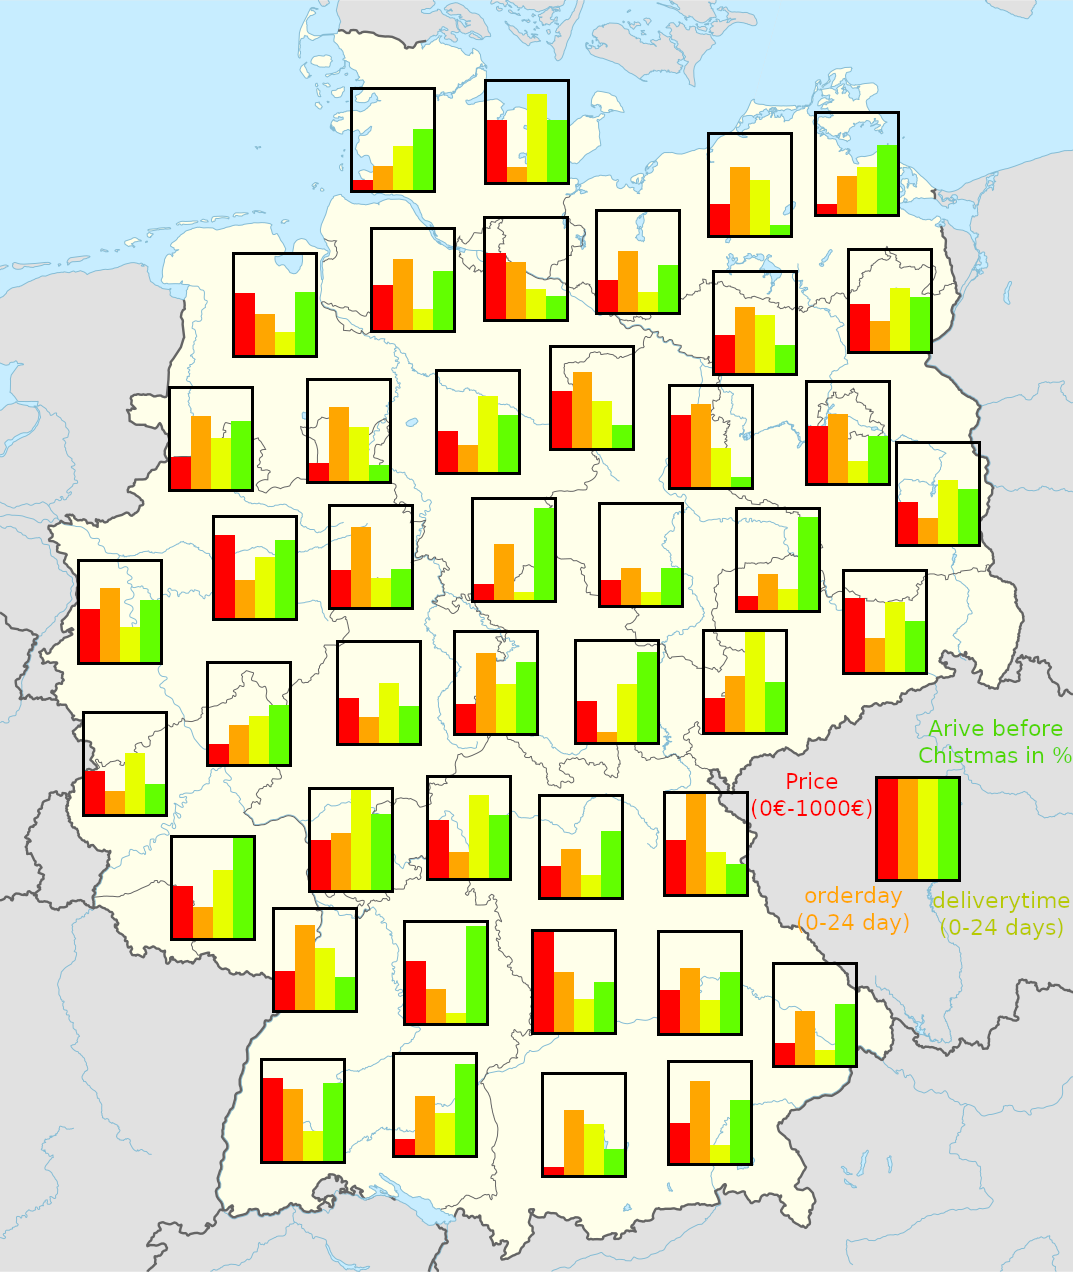
\includegraphics[width=0.7\linewidth]{germany-2b}
	\caption{static visualization}
	\label{fig:germany-2b}
\end{figure}

\begin{enumerate}
	\item average delivery duration per area
	\item average price per area
	\item average day when the order was placed per area
	\item average percentage if order arrived before Christmas per area
\end{enumerate}
\subsection*{c)}

\end{document}
